% coding:utf-8

%----------------------------------------
%FOSAPHY, a LaTeX-Code for a summary of basic physics
%Copyright (C) 2013, Daniel Winz, Ervin Mazlagic

%This program is free software; you can redistribute it and/or
%modify it under the terms of the GNU General Public License
%as published by the Free Software Foundation; either version 2
%of the License, or (at your option) any later version.

%This program is distributed in the hope that it will be useful,
%but WITHOUT ANY WARRANTY; without even the implied warranty of
%MERCHANTABILITY or FITNESS FOR A PARTICULAR PURPOSE.  See the
%GNU General Public License for more details.
%----------------------------------------

\chapter{Reibung}

\newpage

\section{Reibungskraft}
Die Reibungskraft $\vec{F}_R$ ist eine Kraft welche zwischen sich
berührenden Körpern auftritt. Sie ist definiert als das Produkt aus
der Kraft $\vec{F}_N$ welche normal zwischen den Körpern anliegt
und dem Reibungskoeffizienten $\mu$ welcher die 
Oberflächenbeschaffenheit beschreibt. 

\begin{figure}[h!]
	\centering
	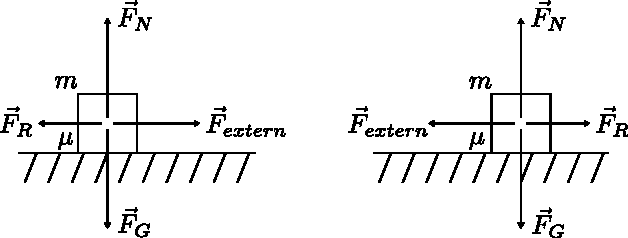
\includegraphics[scale=0.8]{reibung.pdf}
	\caption{Reibungskraft für eine Masse die auf einer Unterlage 
		liegt mit $\sum \vec{F}_{extern}$ positiv (l)
		und negativ (r).}
\end{figure}

\noindent
Die Richtung der Reibungskraft ist dabei stets entgegen der 
anliegenden äusseren Nettokraft 
$\sum \vec{F}_{extern}$.

\[ \boxed{
	\vec{F}_R = \vec{F}_N \cdot \mu
		\qquad ,\vec{F}_R \bot \vec{F}_N
}\]

\section{Bewegungsbedingung}
\noindent
Ein Körper der eine Reibung kennt, bringt eine Kraft $\vec{F}_R$ 
auf entgegen der anliegenden Nettokraft $\sum \vec{F}_{extern}$. 
Das bedeutet, dass ein solcher Körper in Ruhe bleibt, solange die 
anliegende Nettokraft $\sum \vec{F}_{extern} \leq \vec{F}_R$ ist. 
Somit ergibt sich die Bewegungsbedingung zu

\[ \boxed{\begin{array}{l r l}
	\text{Körper bleibt in Ruhe falls } & 
		\sum \vec{F}_{extern} & \leq \vec{F}_R \\
	& & \\
	\text{Körper bewegt sich falls } &
		\sum \vec{F}_{extern} & > \vec{F}_R 
\end{array}} \]

\section{Reibungskoeffizient}
Der Reibungskoeffizient $\mu$ wird typischerweise für zwei Fälle 
angegeben, welche voneinander zu unterscheiden sind.
\begin{itemize}
	\item Haften $\Rightarrow$ Haftreibungskoeffizient $\mu_{HR}$
	\item Gleiten $\Rightarrow$ Gleitreibungskoeffizient $\mu_{GR}$
\end{itemize}

\noindent
Für den Reibungskoeffizienten gilt stets, dass der Koeffizient für die
Haftung grösser oder zumindest gleich ist wie für das Gleiten 
(bei den selben Bedingungen).

\[ \boxed{
	\mu_{HR} \geq \mu_{GR}
}\]

\begin{footnotesize}
\begin{longtable}{llll}
  \rowcolor{white} \textbf{Material 1} & \textbf{Material 2} 
  & \textbf{Haftreibung $\mu_{HR}$} & \textbf{Gleitreibung $\mu_{GR}$}\\
  \rowcolor{lgray}  Stahl     & Stahl             & 0.74 & 0.57\\
  \rowcolor{white}  Aluminium & Stahl             & 0.61 & 0.47\\
  \rowcolor{lgray}  Kupfer    & Stahl             & 0.53 & 0.36\\
  \rowcolor{white}  Messing   & Stahl             & 0.51 & 0.44\\
  \rowcolor{lgray}  Zink      & Grauguss          & 0.85 & 0.21\\
  \rowcolor{white}  Kupfer    & Grauguss          & 1.05 & 0.29\\
  \rowcolor{lgray}  Glas      & Glas              & 0.94 & 0.40\\
  \rowcolor{white}  Kupfer    & Glas              & 0.68 & 0.53\\
  \rowcolor{lgray}  Teflon    & Teflon            & 0.04 & 0.04\\
  \rowcolor{white}  Teflon    & Stahl             & 0.04 & 0.04\\
  \rowcolor{lgray}  Gummi     & Beton (trocken)   & 1.0  & 0.80\\
  \rowcolor{white}  Gummi     & Beton (nass)      & 0.30 & 0.25
\end{longtable}
\end{footnotesize}

